\documentclass[11pt]{article}

\usepackage{times}
\usepackage[utf8]{inputenc} % allow utf-8 input
\usepackage[T1]{fontenc}    % use 8-bit T1 fonts
\usepackage{url}            % simple URL typesetting
\usepackage{graphics}
\usepackage{color}
\usepackage{amsfonts}       % blackboard math symbols
\usepackage{amsmath}       % blackboard math symbols
\usepackage{amssymb}
\usepackage{acronym}
\usepackage{lipsum}
\usepackage{booktabs}
\usepackage{caption}

\usepackage{geometry}
\geometry{left=2.8cm,right=2.8cm,top=2.6cm,bottom=2.6cm}
\usepackage{fancyhdr}
\pagestyle{fancy}
\usepackage{hyperref}% should be the last package you include
\usepackage{graphicx}
\usepackage{todonotes}

\newcommand{\theteam}{}
\newcommand{\team}[1]{\def\theteam{#1}}


\fancyhead[L]{\theteam}
\fancyhead[R]{\thepage}
\cfoot{}

\setlength{\parindent}{0pt}

\team{DRAI: Jannik Rombach, Adriano Polzer}
\title{RL-Course 2025/26: Final Project Report}
\author{\theteam}

\begin{document}
\maketitle

\section{Introduction}\label{sec:intro}

Reinforcement learning in adversarial settings poses unique challenges where an agent 
must not only learn to act effectively, but to do so against an opponent that actively 
counters its behavior. In this work, we train agents for a 1v1 hockey environment 
inspired by air hockey, where two players compete on opposite sides of a rink to 
score goals against each other. The game requires a combination of offensive and 
defensive skills across a fully continuous action space, with scoring goals as 
the ultimate objective.

\medskip
Generalizing across different opponent play styles proves to be the central difficulty. 
We address this through reward shaping to accelerate early learning, exploration 
design, and most importantly a self-play curriculum that progressively challenges the 
agent with a diverse and evolving pool of opponents. We find that the diversity of 
this pool, rather than any single algorithmic choice, is the primary driver of 
agent robustness.

\medskip
We implement and compare two established off-policy algorithms, \ac{TD3} and \ac{SAC}, 
and analyze their behavior under different training conditions. The algorithms are first 
validated on standard continuous control benchmarks before being applied to the hockey 
environment. Methodology is covered in Section~\ref{sec:method}, experimental results 
in Section~\ref{sec:eval}, and conclusions in Section~\ref{sec:discussion}. 
The full code and configuration files are available at 
\url{https://github.com/JannikRom/drai-rl}.
\section{Method}\label{sec:method}

The hockey environment's fully continuous action space makes discrete-action methods such as
\ac{DQN}~\cite{mnih2015human:DQN} inapplicable, and on-policy algorithms such as
\ac{PPO}~\cite{SchulmanEtAl2017:PPO} less attractive due to poor sample efficiency.
We therefore adopt two off-policy, continuous-control algorithms that share a common backbone
yet represent complementary design philosophies: \ac{TD3}~\cite{fujimoto2018:TD3} optimizes a
deterministic policy with explicit bias-correction mechanisms, while \ac{SAC}~\cite{haarnoja2018:SOFT}
optimizes a stochastic policy through entropy maximization.
Both maintain a replay buffer $\mathcal{D}$ of transitions $(s_t, a_t, r_t, s_{t+1}, d_t)$,
train an actor $\pi$ and one or more critics $Q_\theta$ on minibatches from $\mathcal{D}$, and
stabilize learning via slowly updated target networks through Polyak averaging,
\begin{equation}
  \theta' \leftarrow \tau\,\theta + (1-\tau)\,\theta', \qquad
  \phi'   \leftarrow \tau\,\phi  + (1-\tau)\,\phi',
  \label{eq:polyak}
\end{equation}
where $\tau \ll 1$ ensures the target parameters $\theta'$ and $\phi'$ track their online
counterparts $\theta$ and $\phi$ slowly, providing a stable and consistent learning target
throughout training.
The individual algorithms are described in Sections~\ref{sec:td3} and~\ref{sec:sac},
further improvements to both are presented in Section~\ref{sec:improvements}.


\subsection{Twin Delayed Deep Deterministic Policy Gradient}
\label{sec:td3}

\ac{TD3}~\cite{fujimoto2018:TD3} extends \ac{DDPG}~\cite{lillicrap2015:DDPG} by adressing two fundamental failure modes of determenistic actor-critic methods:
overestimation bias in the critic and instability in polciy updates.
The actor encodes a \emph{deterministic} policy $a = \pi_\phi(s)$ and is trained to maximize expected discounted return via the determenistic policy gradient theorem~\cite{silver2014:DPG}:
\begin{equation}
  \nabla_\phi J(\phi)
    \approx \mathbb{E}_{s \sim \mathcal{D}}\!\left[
      \nabla_a Q_{\theta}(s,a)\big|_{a=\pi_\phi(s)}\,
      \nabla_\phi \pi_\phi(s)
    \right].
\end{equation}
In actor-critic methods, the policy is updated greedily with respect to the critic,
meaning any overestimation in the value function is directly exploited by the actor,
leading to suboptimal or diverging behaviour~\cite{fujimoto2018:TD3}.

\ac{TD3} adresses this with three interacting mechanisms.

\vspace{4pt}

\textbf{Clipped double Q-learning}

Two independent critics $Q_{\theta_1}$ and $Q_{\theta_2}$ are trained in parallel but share no parameters.
When computing Bellman targets, the minimum of the two target critics is used:
\begin{equation}
  y = r + \gamma(1-d)\min_{i=1,2} Q_{\theta_i'}(s', \tilde{a})
  \label{eq:td3target}
\end{equation}
where $d$ indicates episode termination and $\theta_i$ are the target network parameters updated via~\eqref{eq:polyak}.
Taking the minimum introduces a conservative bias that counteracts the systematic overastimation inherent in maximizing over noisy function approximators.
Both critics are updated independently by minimizing the mean squarred Bellman error $(y - Q_{\theta_i}(s, a))^2$ over minibatches from $D$.

Since gradients flow independently through each critic, the two networks diverge slightly,
preventing the correlated overestimation that arises when a single critic is used.

\vspace{4pt}

\textbf{Target policy smoothing}

To prevent the actor from exploiting narrow, misleading peaks in the value function, 
the target action is perturbed with clipped Gaussian noise before evaluating the Bellman target:
\begin{equation}
  \tilde{a} = \operatorname{clip}\!\left(\pi_{\phi'}(s') + \epsilon,\;a_{\min},\;a_{\max}\right),
  \quad \epsilon \sim \operatorname{clip}\!\left(\mathcal{N}(0,\sigma),\;-c,\;c\right).
\end{equation}
This encourages the critics to learn a smoother value landscape, making individual erroneous peaks less exploitable.
The noise standard deviation $\sigma$ and clip range $c$ are hyperparameters that control the effective radius of this smoothing.

\vspace{4pt}

\textbf{Delayed policy updates}

Even with conservative targets and smoothed backups, updating the actor at every critic step introduces high variance into the policy gradient:
the critic has not yet fully integrated the latest target information before its gradient is used to move the policy.
\ac{TD3} therefore updates the actor every $K$ critic steps, typically $K=2$.
This delay ensures the critics are in a more stable and accurate state when the actor gradient is computed,
substantially reducing variance of policy updates and preventing the actor from over-adapting to transient critic errors~\cite{fujimoto2018:TD3}.
Target networks for both actor and critics are updated via the shared Polyak rule~\eqref{eq:polyak}, 
ensuring the learning targets change slowly and the training signal remains consistent across consecutive gradient steps.

Togehter, these three mechanisms directy counteract the core failure modes of deteremenistic actor-critic methods:
clipped double Q-learning reduces overestimation bias, target policy smoothing regularizes the value function against sharp local peaks,
and delayed updates reduce gradient variance during policy optimization.

\subsection{Soft Actor-Critic}
\label{sec:sac}

\ac{SAC} is an off-policy actor-critic algorithm designed for optimizing \emph{stochastic} policies in
continuous action spaces.
Our implementation follows the framework introduced by~\cite{haarnoja2018:SOFT}, which augments the
standard maximum reward objective with an entropy maximization term~\cite{ziebart2010}.
This approach encourages wider exploration and improves robustness by seeking a policy that
maximizes the trade-off between expected return and entropy:
\begin{equation}
  J(\pi) = \sum_{t=0}^{T}
    \mathbb{E}_{(\mathbf{s}_t,\mathbf{a}_t)\sim\rho_\pi}\!\left[
      r(\mathbf{s}_t,\mathbf{a}_t) + \alpha\,\mathcal{H}\!\left(\pi(\cdot|\mathbf{s}_t)\right)
    \right]
\end{equation}
where $\rho_\pi$ denotes the state-action distribution induced by policy $\pi$ and $\mathcal{H}$
represents the entropy of the policy at state $\mathbf{s}_t$.

The \ac{SAC} algorithm consists of an actor, critic, and an entropy regularization term governed
by a temperature parameter $\alpha$.
The actor is parameterized by a neural network that defines a Gaussian distribution over the
continuous action space by estimating the mean $\mu_\theta(s)$ and standard deviation
$\sigma_\theta(s)$ in its output layer.

To ensure differentiability of the sampling process with respect to the policy parameters, the
reparameterization trick is applied~\cite{haarnoja2018:SOFT, kingma2014auto}.
Instead of sampling actions directly from the Gaussian distribution, actions are expressed as
$a = \mu_\theta(s) + \sigma_\theta(s) \odot \epsilon$ where $\epsilon \sim \mathcal{N}(0, I)$ is
a standard normal random variable.

The sampled actions are passed through a $\tanh$ function and scaled to match the action bounds
of the environment.
To correctly account for this squashing transformation in the entropy term, the log-probability
is adjusted using the determinant of the Jacobian of the $\tanh$ transformation.
The actor is trained on the maximum entropy objective~\cite{haarnoja2018:SOFT}:
\begin{equation}
  J(\pi_\phi) =
    \mathbb{E}_{(\mathbf{s}_t \sim \mathcal{D})}\!\left[
      \mathbb{E}_{(\mathbf{a}_t) \sim \pi_\phi}\!\left[
        \alpha \log \pi_\phi(a_t|s_t) - Q_\theta(s_t, a_t)
      \right]
    \right]
\end{equation}
where for each state sampled from the replay buffer $\mathcal{D}$, an action is sampled from the
actor and the critic estimates the value for each state-action pair.

As presented in the follow-up work~\cite{haarnoja2018algorithms}, we employ two Q-networks for
the critic instead of a single Q-network and a value network as originally proposed.
The soft value function can be implicitly derived from the soft Q-function by combining the
Q-values with the policy entropy term.

During training, two independent Q-networks estimate the value of a state-action pair.
To mitigate overestimation bias, soft policy evaluation is performed using the minimum of the two
Q-values, which provides a more conservative value estimate~\cite{fujimoto2018:TD3}.
The critic is trained using a mean squared Bellman error loss:
\begin{equation}
  J_Q(\theta_i) = \mathbb{E}_{\mathcal{D}}\!\left[
    \left(Q_{\theta_i}(s_t,a_t) - y_t\right)^2
  \right]
\end{equation}
with target value
\begin{equation}
  y_t = r_t + \gamma\!\left(
    \min_{j=1,2} Q_{\bar{\theta}_j}(s_{t+1},a_{t+1})
    - \alpha \log \pi_\phi(a_{t+1}|s_{t+1})
  \right).
\end{equation}
The target networks $\bar{\theta}_j$ are updated using soft updates with factor $\tau$, which
improves training stability by preventing rapid divergence between online and target critics.

Furthermore, automatic parameter tuning is implemented as introduced in the follow-up
paper~\cite{haarnoja2018algorithms}.
The temperature parameter $\alpha$ is optimized to match a target policy entropy, allowing the
agent to automatically balance exploration and exploitation.
The temperature is updated by minimizing
\begin{equation}
  J(\alpha) = \mathbb{E}_{a_t \sim \pi_\phi}\!\left[
    -\alpha\left(\log \pi_\phi(a_t|s_t) + \bar{\mathcal{H}}\right)
  \right],
\end{equation}
where $\bar{\mathcal{H}}$ denotes the target entropy, typically set to
$-\operatorname{dim}(\mathcal{A})$ as recommended in~\cite{haarnoja2018algorithms}.
The parameter $\alpha$ is optimized using a gradient-based method.




\subsection{Improvements}
\label{sec:improvements}

We implemented a framework based on YAML configuration files to manage and persist training runs,
enabling reproducible experiments and systematic tracking of hyperparameter changes.
All modifications described below are applied on top of both the \ac{TD3} and \ac{SAC} base implementations.


\subsubsection*{Replay Buffer}
Since both implemented algorithms are off-policy, training relies on data stored in a replay
buffer. We implemented standard \ac{ER}, which improves data efficiency by reusing past 
interactions and reducing correlations between subsequent samples. Transitions are stored as 
tuples $(s_t, a_t, r_t, s_{t+1})$ in a finite buffer; during training, batches are sampled 
uniformly from the buffer. However, uniform sampling treats all transitions equally, while 
transitions with large \ac{TD} errors may provide stronger learning signal. To address this 
limitation, we additionally implement \ac{PER}.

\ac{PER} assigns higher sampling probabilities to transitions with larger \ac{TD} 
errors~\cite{Schaul2015PrioritizedER}. Each transition $i$ is associated with a priority 
value $p_i = |\delta_i| + \varepsilon$, where $\delta_i$ denotes the \ac{TD} error and 
$\varepsilon > 0$ ensures non-zero probability. Transitions are sampled according to
\begin{equation}   
  P(i) = \frac{p_i^\alpha}{\sum_k p_k^\alpha}, 
\end{equation}
where $\alpha$ determines the degree of prioritization ($\alpha = 0$ recovers uniform 
sampling). Prioritized sampling introduces a bias into the gradient estimates, corrected 
via importance-sampling weights:
\begin{equation}   
  w_i = \left(\frac{1}{N} \cdot \frac{1}{P(i)}\right)^\beta, 
\end{equation}
where $N$ is the buffer size and $\beta$ controls the strength of bias 
correction~\cite{Schaul2015PrioritizedER}. To ensure asymptotically unbiased updates, 
$\beta$ is annealed linearly to $1$ over a configurable fraction of total training steps. 
Efficient sampling and priority updates are implemented using a binary SumTree data 
structure, enabling both operations in $\mathcal{O}(\log N)$ time.

\subsubsection*{Pink Noise}
Exploration in off-policy algorithms is commonly achieved by injecting noise into the 
actor's actions during training. The standard choice is white noise $\mathcal{N}(0, \sigma)$, 
which is temporally uncorrelated, meaning each noise sample is drawn independently at 
every timestep, leading to jittery exploration with no coherence across consecutive actions. 
Eberhard et al. introduced colored noise as a principled alternative, parameterized by a 
spectral exponent $\beta$ that controls the degree of temporal correlation~\cite{eberhard2023pink}. 
Increasing $\beta$ yields smoother trajectories where the noise is correlated with past samples, 
encouraging the agent to commit to exploratory directions over multiple consecutive steps. 
Pink noise ($\beta = 1$) was shown to strike the best balance between exploitation and 
exploration across a range of continuous control tasks~\cite{eberhard2023pink}.

Colored noise is generated by decomposing a white noise signal into its frequency components 
via the Fast Fourier Transform, scaling each component $f$ by $f^{-\beta/2}$, and transforming 
the result back into the time domain, where frequency refers to how rapidly the noise changes 
over consecutive timesteps. Suppressing high frequencies and amplifying low frequencies 
produces a noise sequence that varies slowly over time, resulting in temporally correlated 
action perturbations across the agent's trajectory. We apply pink noise as the exploration 
noise for \ac{TD3}, replacing the standard Gaussian perturbation. Since \ac{SAC} learns a 
stochastic policy whose entropy is explicitly regularized through $\alpha$, it does not rely 
on external exploration noise and pink noise is therefore not applicable.

\subsubsection*{Reward Shaping}
To enhance learning in the hockey environment, we extend the default reward formulation 
with additional shaping terms. The environment provides a sparse reward for winning, a 
penalty for losing, and optional signals for puck contact and puck velocity direction, 
which are not enabled by default. The total reward is given by $r = \sum_{i} w_i \cdot r_i$,
where each $r_i$ denotes a reward component and $w_i \in \mathbb{R}$ its corresponding weight.

In early training stages, the agent often required a significant number of timesteps 
before initiating contact with the puck. To accelerate early learning, we introduce a 
time-penalty term $r_{\text{passive}}$, applied when the puck remains stationary on the 
agent's side of the field beyond the first $10\%$ of episode steps,
\begin{equation}
    r_{\text{passive}}(t) = \begin{cases} -c & \text{if } x_{\text{puck}} \leq 0, \; 
    \|v_{\text{puck}}\| < 0.1, \text{ and } t > 0.1 \cdot T_{\max}, \\ 
    0 & \text{otherwise,} \end{cases}
\end{equation}
where $c > 0$ is a configurable penalty coefficient. To encourage defensive positioning, 
we additionally reward the agent for staying close to its own goal when the puck is on 
the opponent's side,
\begin{equation}
    r_{\text{defense}} = \begin{cases} \dfrac{1}{1 + \|p_{\text{agent}} - g\|_2} 
    & \text{if } x_{\text{puck}} > 0, \\ 0 & \text{otherwise,}\end{cases}
\end{equation}
where $g$ denotes the agent's goal center. All shaping components are individually 
configurable via the YAML configuration file and can be freely weighted or disabled.


\subsubsection*{Self-Play}


\begin{figure}[htbp]
\centering
\includegraphics[width=0.85\textwidth]{./figures/selfplay_diagram.pdf}
\caption{Self-play opponent pool workflow (AlphaZero-inspired). Future extension for TD3.}
\label{fig:selfplay}
\end{figure}

\section{Evaluation}\label{sec:eval}

\subsection{Simple Environments}


\subsection{Hockey Environment}

Own vs. Standard


Self Play

\section{Discussion}
\label{sec:discussion}

Both SAC and TD3 proved to be well-suited algorithms for the hockey environment. SAC 
converged faster and required less manual tuning due to its automatic entropy 
regularization, while TD3 with pink noise exploration provided a competitive alternative. 
Hyperparameter tuning required considerable effort, but the most significant performance 
gains ultimately came from longer training runs and exposure to diverse opponents rather 
than from any single algorithmic choice.

The modular YAML-based framework proved valuable throughout the project, allowing rapid 
iteration over configurations without code changes. Combined with TensorBoard logging, 
we maintained a clear picture of training progression at all times. The round-robin 
tournament with TrueSkill ranking provided a reliable and interpretable comparison 
across all agent variants at every stage of development.

\medskip
The most impactful finding was that training against a diverse pre-trained opponent pool 
led to substantially stronger and more generalizable agents. Agents trained only against 
the basic opponents or against pure self-play snapshots tended to overfit quickly, 
converging to narrow strategies that exploited specific weaknesses of familiar opponents. 
This overfitting became apparent only through the tournament, where top-ranked agents 
unexpectedly lost to stylistically different lower-ranked opponents. The final SAC and 
TD3 agents trained against the pre-trained pool win consistently against both the weak 
and strong basic opponent, as reflected in the win rates reported in 
Table~\ref{tab:tournament_results} in the appendix. In hindsight, we would have invested 
more time earlier in building a larger and more varied pool, including agents trained 
under more diverse configurations and potentially additional algorithm types, to capture 
an even broader range of play styles.

Our results strongly suggest that exposure to diverse opponents is the primary driver of 
generalization. For the live tournament against the other course participants, fine-tuning 
against recorded opponent trajectories between matches could therefore be a particularly 
effective strategy to gain ranking, as it would allow the agent to adapt directly to the 
playing styles encountered in the competition.

\medskip
Overall, the project offered valuable practical insight into the challenges of 
reinforcement learning that goes well beyond theoretical study alone. The hands-on 
nature of iteratively training, analyzing games, and refining strategies made the 
underlying complexity of the problem genuinely concrete. The infrastructure built 
around the training pipeline provided a solid foundation that made this iterative 
process efficient, reproducible, and enjoyable.
\bibliographystyle{abbrv}
\bibliography{literatur}

\newpage
\appendix



\section{Simple Environment Diagnostics}
\subsection{Training Curves}

Bla Bla
Hier auch allgemein text und vlt. Hyperparameter

\subsection{Training Curves}
\label{app:simple_losses}

Bla Bla Bla Bla

Sui Sui Sui

\subsubsection{Pendulum}
Further training diagnostics for the Pendulum environment are shown in Figure~\ref{fig:pendulum_losses}. 
The SAC entropy temperature $\alpha$ decays steadily, reflecting increasing policy confidence. 
TD3 losses stabilize toward the end of training.

\begin{figure}[htbp]
\centering
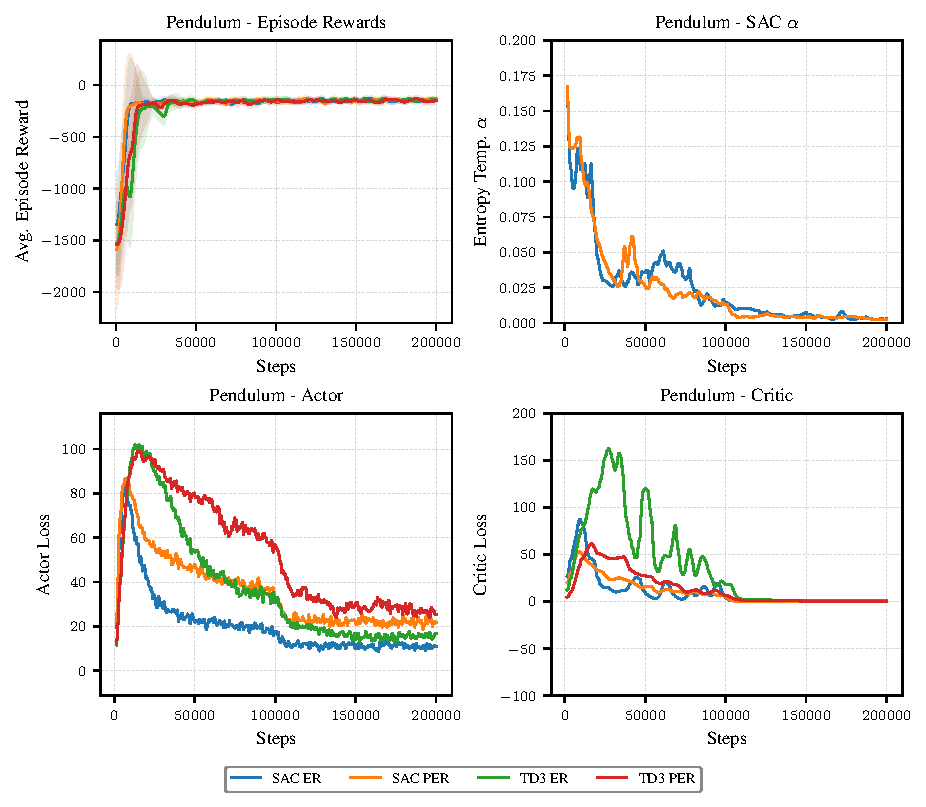
\includegraphics[width=\textwidth]{figures/overview_pendulum.pdf}
\caption{Training diagnostics for Pendulum environment. 
    Top left: average episode reward. Top right: SAC entropy temperature $\alpha$. 
    Bottom left: actor loss. Bottom right: critic loss.}
\label{fig:pendulum_losses}
\end{figure}

\newpage

\subsubsection{Lunar Lander}
Training diagnostics for Lunar Lander are shown in Figure~\ref{fig:lunarlander_losses}. 
Both algorithms show stable convergence, with TD3 exhibiting smoother critic losses.

\begin{figure}[htbp]
\centering
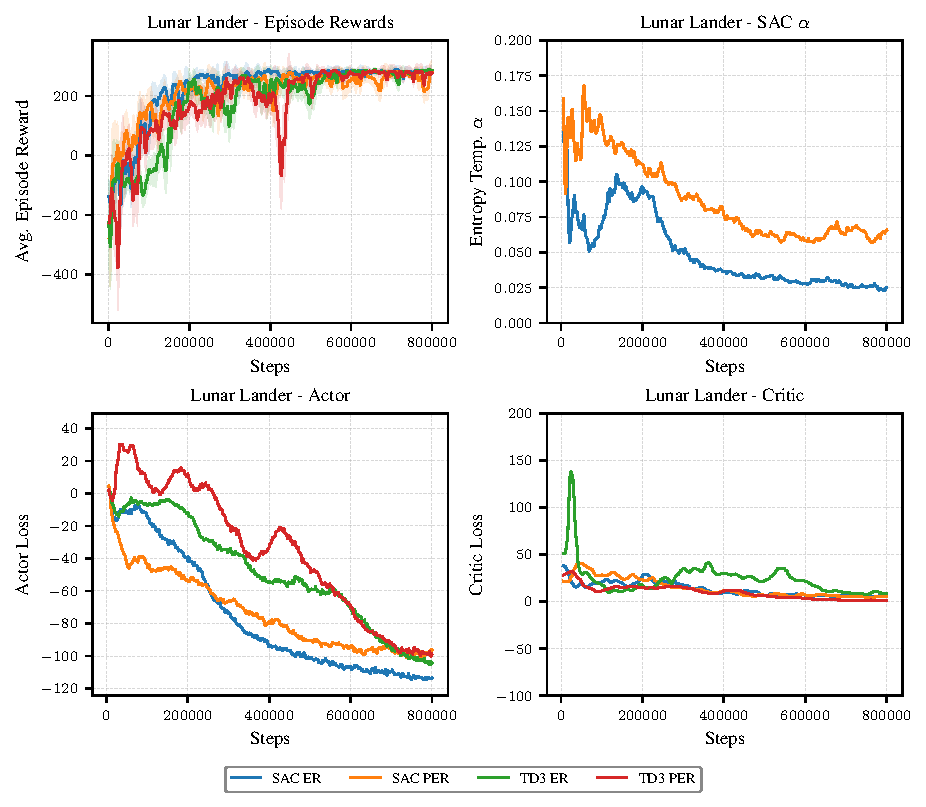
\includegraphics[width=\textwidth]{figures/overview_lunar_lander.pdf}
\caption{Training diagnostics for Lunar Lander environment. 
    Top left: average episode reward. Top right: SAC entropy temperature $\alpha$. 
    Bottom left: actor loss. Bottom right: critic loss.}
\label{fig:lunarlander_losses}
\end{figure}

\newpage

\subsubsection{Half Cheetah}
Half Cheetah diagnostics are shown in Figure~\ref{fig:halfcheetah_losses}. 
The higher-dimensional action space leads to slower convergence, but both variants 
achieve stable performance.

\begin{figure}[htbp]
\centering
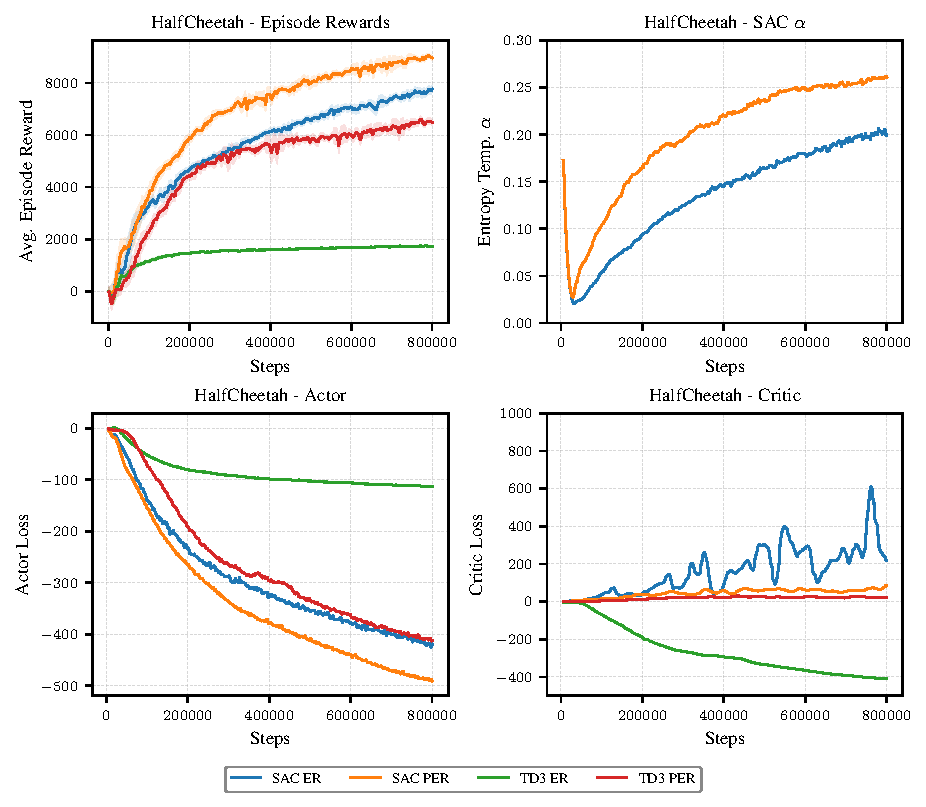
\includegraphics[width=\textwidth]{figures/overview_half_cheetah.pdf}
\caption{Training diagnostics for Half Cheetah environment. 
    Top left: average episode reward. Top right: SAC entropy temperature $\alpha$. 
    Bottom left: actor loss. Bottom right: critic loss.}
\label{fig:halfcheetah_losses}
\end{figure}


\subsubsection{Pendulum}
%plot
\subsubsection{Lunar Lander}
%plot
\subsubsection{Half Cheetah}
%plot
\subsection{Hyperparameters}
\label{app:simple_parameters}
\begin{table}[htbp]
\centering
\caption{Hyperparameters used across algorithms.}
\label{tab:hyperparams_all}

\begin{tabular}{lcccc}
\toprule
\textbf{Parameter} 
& \textbf{SAC} 
& \textbf{SAC}
& \textbf{TD3}
& \textbf{TD3} \\
\midrule

Replay buffer type
& ER & PER & ER & PER \\


Discount factor $\gamma$
& 0.98 & 0.98 & 0.98 & 0.98 \\

Actor learning rate
& $3\times10^{-4}$ & $3\times10^{-4}$ 
& $3\times10^{-4}$ & $3\times10^{-4}$ \\

Critic learning rate
& $3\times10^{-4}$ & $3\times10^{-4}$ 
& $3\times10^{-4}$ & $3\times10^{-4}$ \\

Entropy coefficient $\alpha$
& 0.2 & 0.2 & -- & -- \\

Replay buffer size
& $10^6$ & $10^6$ & $10^6$ & $10^6$ \\

Noise
& -- & -- & 
$\sigma=0.2$, \newline clip=0.5 
& $\sigma=0.2$, \newline clip=0.5 \\

Network architecture
& $[512,256]$ & $[512,256]$ 
& $[512,256]$ & $[512,256]$ \\

Critic architecture
& $[512,256,128]$ & $[512,256,128]$ 
& $[512,256,128]$ & $[512,256,128]$ \\

\bottomrule
\end{tabular}
\end{table}

%table


\newpage
\section{Hockey Environment Diagnostics}
sadshjashdjhaskjdhkjashdkjhaskjdhjasho ihchsaklhekhkjshdjkbawnbdwbdiuabkjbdw buiasijcbkjawbjhbjhbjchvbajwhbvjhd
sadshjashdjhaskjdhkjashdkjhaskj dhjashoihchsaklhek hkjshdjkbawnbdwbdiuabkjbd buiasijcbkjawbjhbjhbjchvbajwhbvjhd


\subsection{Training Curves}
\label{app:hockey_curves}

Further training diagnostics are shown in Figure~\ref{fig:hockey_losses}. The SAC 
entropy temperature $\alpha$ decays steadily for both variants, reflecting increasing 
policy confidence. The TD3 actor losses decrease monotonically into negative territory 
as the actor learns to maximize the critic's Q-values. The critic loss of TD3 Basic 
appears noisier than the other variants, which may be attributable to the uncorrelated 
white noise producing more inconsistent transition patterns in the replay buffer. 
Critic losses decrease across all variants towards the end of training, indicating 
stable convergence.

\begin{figure}[htbp]
\centering
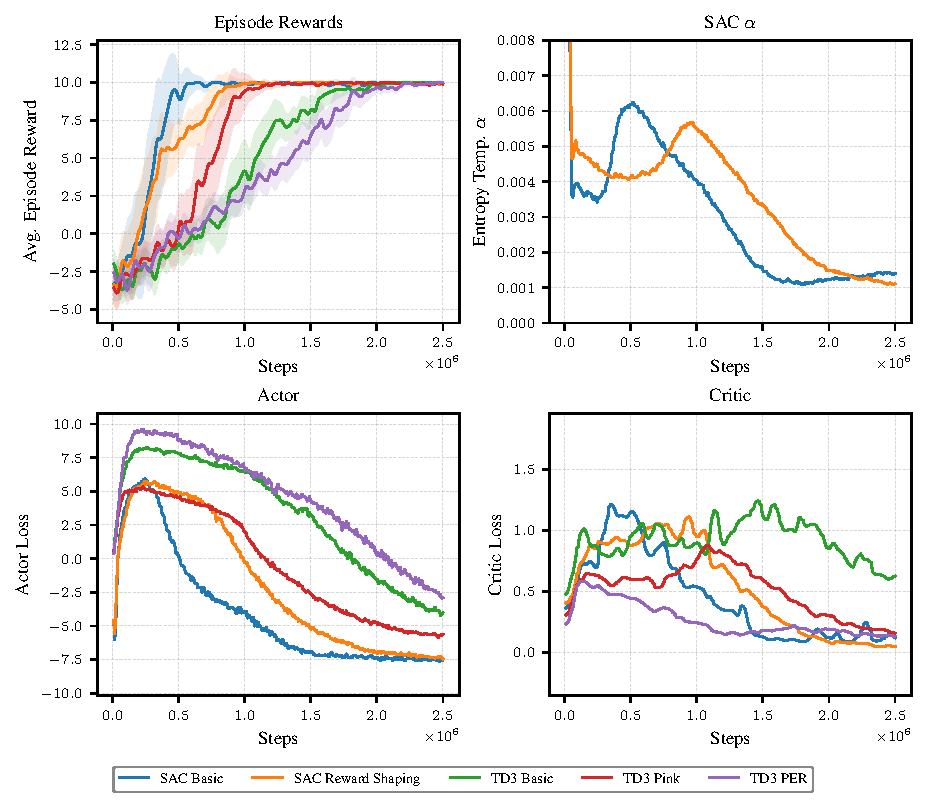
\includegraphics[width=\textwidth]{figures/3_2_overview_plot.pdf}
\caption{Training diagnostics for selected hockey environment configurations. 
    Top left: average episode reward. Top right: SAC entropy temperature $\alpha$. 
    Bottom left: actor loss. Bottom right: critic loss.}
\label{fig:hockey_losses}
\end{figure}


\subsection{Hyperparameters}

\vspace{+0.6cm}

\begin{table}[htbp]
\centering
\caption{SAC hyperparameters.}
\vspace{-0.3cm}
\label{tab:sac_hyperparams}
\begin{tabular}{lc}
\toprule
\textbf{Hyperparameter} & \textbf{Value} \\
\midrule
Discount factor $\gamma$         & $0.98$ \\
Soft update $\tau$               & $0.005$ \\
Actor learning rate              & $3 \times 10^{-4}$ \\
Critic learning rate             & $3 \times 10^{-4}$ \\
$\alpha$ learning rate           & $1 \times 10^{-4}$ \\
Initial entropy coefficient $\alpha$ & $0.2$ \\
Target entropy                   & $-|\mathcal{A}|$ \\
Actor architecture               & $[512, 256]$ \\
Critic architecture              & $[512, 256, 128]$ \\
Replay buffer size               & $10^6$ \\
Batch size                       & $256$ \\
Learning starts                  & $10{,}000$ \\
Reward shaping: touch puck       & $0.1$ \\
Reward shaping: puck direction   & $0.05$ \\
\bottomrule
\end{tabular}
\end{table}

\vspace{+0.6cm}

\begin{table}[htbp]
\centering
\caption{TD3 hyperparameters.}
\vspace{-0.3cm}
\label{tab:td3_hyperparams}
\begin{tabular}{lc}
\toprule
\textbf{Hyperparameter} & \textbf{Value} \\
\midrule
Discount factor $\gamma$         & $0.98$ \\
Soft update $\tau$               & $0.005$ \\
Actor learning rate              & $3 \times 10^{-4}$ \\
Critic learning rate             & $3 \times 10^{-4}$ \\
Policy noise $\sigma$            & $0.2$ \\
Noise clip                       & $0.5$ \\
Policy delay                     & $2$ \\
Exploration noise (pink, $\beta=1$) & $0.15$ \\
Actor architecture               & $[256, 256, 256]$ \\
Critic architecture              & $[256, 256, 128]$ \\
Replay buffer size               & $10^6$ \\
Batch size                       & $256$ \\
Learning starts                  & $10{,}000$ \\
Reward shaping: touch puck       & $0.1$ \\
Reward shaping: puck direction   & $0.05$ \\
\bottomrule
\end{tabular}
\end{table}







\newpage
\section*{List of Acronyms}
\begin{acronym}
\acro{DQN}{Deep Q-Network}
\acro{PPO}{Proximal Policy Optimization}
\acro{DDPG}{Deep Deterministic Policy Gradient}
\acro{TD3}{Twin Delayed Deep Deterministic Policy Gradient}
\acro{SAC}{Soft Actor-Critic}
\acro{ER}{Experience Replay}
\acro{PER}{Prioritized Experience Replay}
\acro{TD}{Temporal Difference}
\end{acronym}

\end{document}
